\documentclass[border=2pt]{standalone}
\usepackage[T1]{fontenc}
\usepackage{lmodern}
\usepackage{tikz}
\usetikzlibrary{arrows.meta,shapes.misc,shapes.geometric,positioning,fit,backgrounds,calc}
\renewcommand{\familydefault}{\sfdefault}
\hyphenpenalty=10000 \exhyphenpenalty=10000
\newcommand{\psClaimFont}{\fontsize{8.80}{10.56}\selectfont\bfseries}
\newcommand{\psSpineFont}{\fontsize{8.20}{9.84}\selectfont}
\newcommand{\psFocalFont}{\fontsize{8.20}{9.84}\selectfont\bfseries}
\newcommand{\psNoteFont}{\fontsize{7.60}{9.12}\selectfont}
\definecolor{psCanvas}{HTML}{F7F3E8}
\definecolor{psInk}{HTML}{20252B}
\definecolor{psCool}{HTML}{4F7CAC}
\definecolor{psWarm}{HTML}{E09F3E}
\definecolor{psAlert}{HTML}{D96855}
\tikzset{
  ps base/.style={align=center, text=psInk, font=\psSpineFont, inner sep=4pt},
  ps operator/.style={ps base, rectangle, rounded corners=3pt, draw=psCool,
    fill=psCool!14, line width=1.5pt},
  ps state/.style={ps base, rectangle, rounded corners=8pt, draw=psInk!60, fill=psInk!7,
    line width=1.3pt},
  ps focal/.style={ps base, rectangle, rounded corners=5pt, draw=psAlert, fill=psWarm!32,
    line width=1.8pt, font=\psFocalFont},
  ps evidence/.style={ps base, rectangle, draw=psInk!45, fill=white,
    line width=1.3pt, font=\psNoteFont},
  ps context/.style={ps base, font=\psNoteFont, text=psInk!75, align=left, inner sep=2pt},
  ps group/.style={rectangle, rounded corners=6pt, fill=psCool!7, draw=psCool!30,
    line width=0.8pt, inner sep=5pt},
  ps claim/.style={font=\psClaimFont, text=psInk, align=left, inner sep=0pt},
  ps primary/.style={draw=psInk, line width=1.9pt, -{Stealth[length=3.0mm, width=2.6mm]}},
  ps secondary/.style={draw=psInk!50, line width=1.4pt, -{Stealth[length=2.4mm, width=2.1mm]}},
  ps data/.style={},
  ps supervision/.style={dash pattern=on 5pt off 3pt},
  ps feedback/.style={bend left=40},
  ps inhibition/.style={-{Bar[width=3.4mm]}},
  ps edge label/.style={font=\psNoteFont, text=psInk!80, fill=white, inner sep=1.5pt},
}
\begin{document}
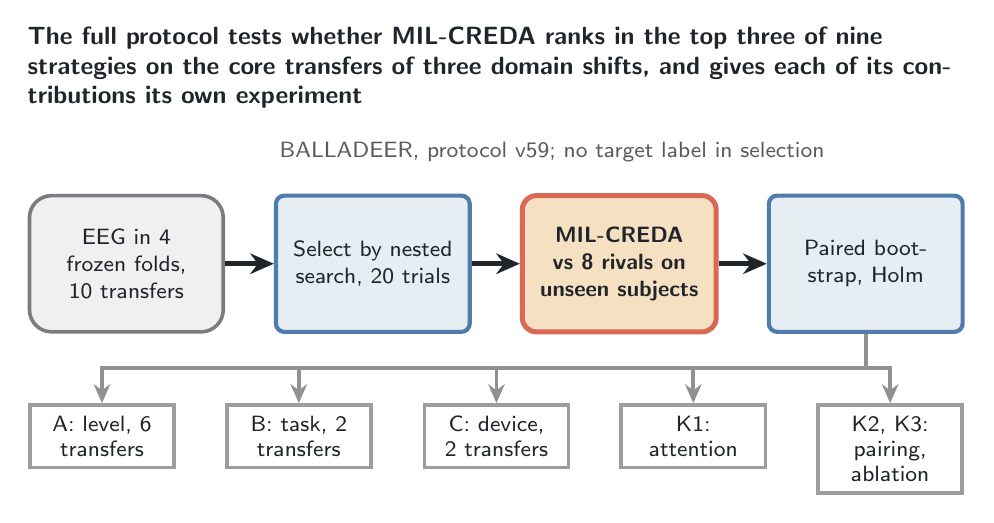
\begin{tikzpicture}
% figure claim: The full protocol tests whether MIL-CREDA ranks in the top three of nine strategies on the core transfers of three domain shifts, and gives each of its contributions its own experiment
% printed width: 345.0pt of a 10pt body (main.tex:fallback); fonts {'claim': 8.8, 'spine': 8.2, 'note': 7.6}
\node[ps state, text width=2.18cm, minimum height=1.73cm, anchor=center] (data) at (1.26,0.00) {EEG in 4 frozen folds, 10 transfers};
\node[ps operator, text width=2.18cm, minimum height=1.73cm, anchor=center] (search) at (4.39,0.00) {Select by nested search, 20 trials};
\node[ps focal, text width=2.18cm, minimum height=1.73cm, anchor=center] (compare) at (7.52,0.00) {MIL-CREDA vs 8 rivals on unseen subjects};
\node[ps operator, text width=2.18cm, minimum height=1.73cm, anchor=center] (tests) at (10.65,0.00) {Paired bootstrap, Holm};
\node[ps evidence, text width=1.55cm, anchor=north] (a) at (0.95,-1.77) {A: level, 6 transfers};
\node[ps evidence, text width=1.55cm, anchor=north] (b) at (3.45,-1.77) {B: task, 2 transfers};
\node[ps evidence, text width=1.55cm, anchor=north] (c) at (5.96,-1.77) {C: device, 2 transfers};
\node[ps evidence, text width=1.55cm, anchor=north] (k1) at (8.46,-1.77) {K1: attention};
\node[ps evidence, text width=1.55cm, anchor=north] (k23) at (10.96,-1.77) {K2, K3: pairing, ablation};
\node[ps context, text width=7.00cm, anchor=south west] (note) at (3.13,1.22) {BALLADEER, protocol v59; no target label in selection};
\coordinate (ps top) at (current bounding box.north);
\node[ps claim, anchor=south west, text width=11.91cm] at ($(0,0 |- ps top)+(0,0.35)$) {The full protocol tests whether MIL-CREDA ranks in the top three of nine strategies on the core transfers of three domain shifts, and gives each of its contributions its own experiment};
\draw[ps primary, ps data] (data.east) -- (search.west);
\draw[ps primary, ps data] (search.east) -- (compare.west);
\draw[ps primary, ps data] (compare.east) -- (tests.west);
\draw[ps secondary, ps data] (tests.south) -- (tests.south |- 0,-1.32) -| (a.north);
\draw[ps secondary, ps data] (tests.south) -- (tests.south |- 0,-1.32) -| (b.north);
\draw[ps secondary, ps data] (tests.south) -- (tests.south |- 0,-1.32) -| (c.north);
\draw[ps secondary, ps data] (tests.south) -- (tests.south |- 0,-1.32) -| (k1.north);
\draw[ps secondary, ps data] (tests.south) -- (tests.south |- 0,-1.32) -| (k23.north);
\end{tikzpicture}
\end{document}
